\documentclass[
	a4paper,10pt
]{scrartcl}

%%% PACKAGES %%%

% PDF/A Compliance
\usepackage[a-2b]{pdfx}

% add unicode support and use german as language
\usepackage[utf8]{inputenc}
\usepackage[ngerman]{babel}

% Use Helvetica as font
\usepackage[scaled]{helvet}
\renewcommand\familydefault{\sfdefault}

% Better tables
\usepackage{tabularx}

% Better enumerisation env
\usepackage{enumitem}

% Use graphics
\usepackage{graphicx}

% Have subfigures and captions
\usepackage{subcaption}

% Be able to include PDFs in the file
\usepackage{pdfpages}

% Have custom abstract heading
\usepackage{abstract}

% Need a list of equation
\usepackage{tocloft}
\usepackage{ragged2e}

% Better equation environment
\usepackage{amsmath}

% Symbols for most SI units
\usepackage{siunitx}

\usepackage{csquotes}

% Clickable Links to Websites and sections
\usepackage{hyperref}

% Change page rotation
\usepackage{pdflscape}

% Symbols like checkmark
\usepackage{amssymb}
\usepackage{pifont}

\usepackage{float}

\usepackage[absolute]{textpos}

% Change line spacing
\renewcommand{\baselinestretch}{0.9}

%%% PATH DEFINITIONS %%%
\graphicspath{{./img/}}

%%% DOCUMENT %%%

\begin{document}

\pagenumbering{gobble}

\begin{textblock*}{5cm}[0,0](15cm,0.7cm)
	
\includegraphics[keepaspectratio,width=5cm]{img/HSLU_Logo}
\end{textblock*}

\vspace*{2cm}

\noindent
\textbf{\LARGE{Untersuchung der Performanz des Invisible Internet Protocols (I2P)}} \\

\vspace{0.5em}

\bgroup
% Remove padding of the table
\setlength\tabcolsep{0cm}

% Table itself
\begin{large}
\noindent
\begin{tabularx}{\textwidth}{p{5cm}X}
    \textbf{Themenbereiche:} & ICT-Infrastrukturen, Security/Privacy,
                    Softwareerstellung, I2P-Netzwerk \\
	\textbf{Student:} & Moritz Küttel\\
	\textbf{Betreuungsperson:} & Dr. Dieter Arnold, HSLU\\
	\textbf{Experte:} & Urs Rufer, TerreActive AG\\
    \textbf{Auftraggebende:} & Carolyn 
    \& Konrad Bächler, DIVA.EXCHANGE\\
	\textbf{Keywords:} & I2P, Netzwerke, Teststand, Performanz, Infrastruktur, Security, Privacy, Anonymität \\
\end{tabularx}
\end{large}
\egroup

\section{Aufgabenstellung}

Der Verein DIVA.EXCHANGE entwickelt einen Software-Prototypen für eine Handelsplattform, um digitale Werte auszutauschen.
Die Handelsplattform soll vollkommen verteilt sein, sowie die Sicherheit und die Privatsphäre der Benutzer sicherstellen.
Es sollen digitale Werte ausgetauscht werden können, ohne sich kennen oder vertrauen zu müssen.
Um dies umzusetzen, wurde auf das Anonymisierungsnetzwerk ``Invisible Internet Protocol'' (I2P) als Grundstein auf der Netzwerkebene gesetzt.
Jedoch hat die Anonymität, Privatsphäre und Sicherheit, die durch I2P geboten wird, ihren Preis: Performanz.
In dieser Arbeit soll empirisch untersucht werden, unter welchen Umständen sich die Performanz des I2P-Netzwerks verbessert.
Insbesondere wurden die Latenzzeiten von TCP-Nachrichten untersucht.

\section{Vorgehen}

Damit die Performance-Messungen empirisch durchgeführt werden konnten, wurde ein Teststand erstellt.
Die Infrastruktur des Teststands wurde als Code abgelegt, damit die Messungen reproduziert werden können.
In einem privaten I2P-Netzwerk können Messungen und Tests ohne äussere Einflüsse ausgeführt werden.
Der Aufbau des Testnetzwerks wird in der folgenden Abbildung schematisch dargestellt:


\begin{figure}[H]
  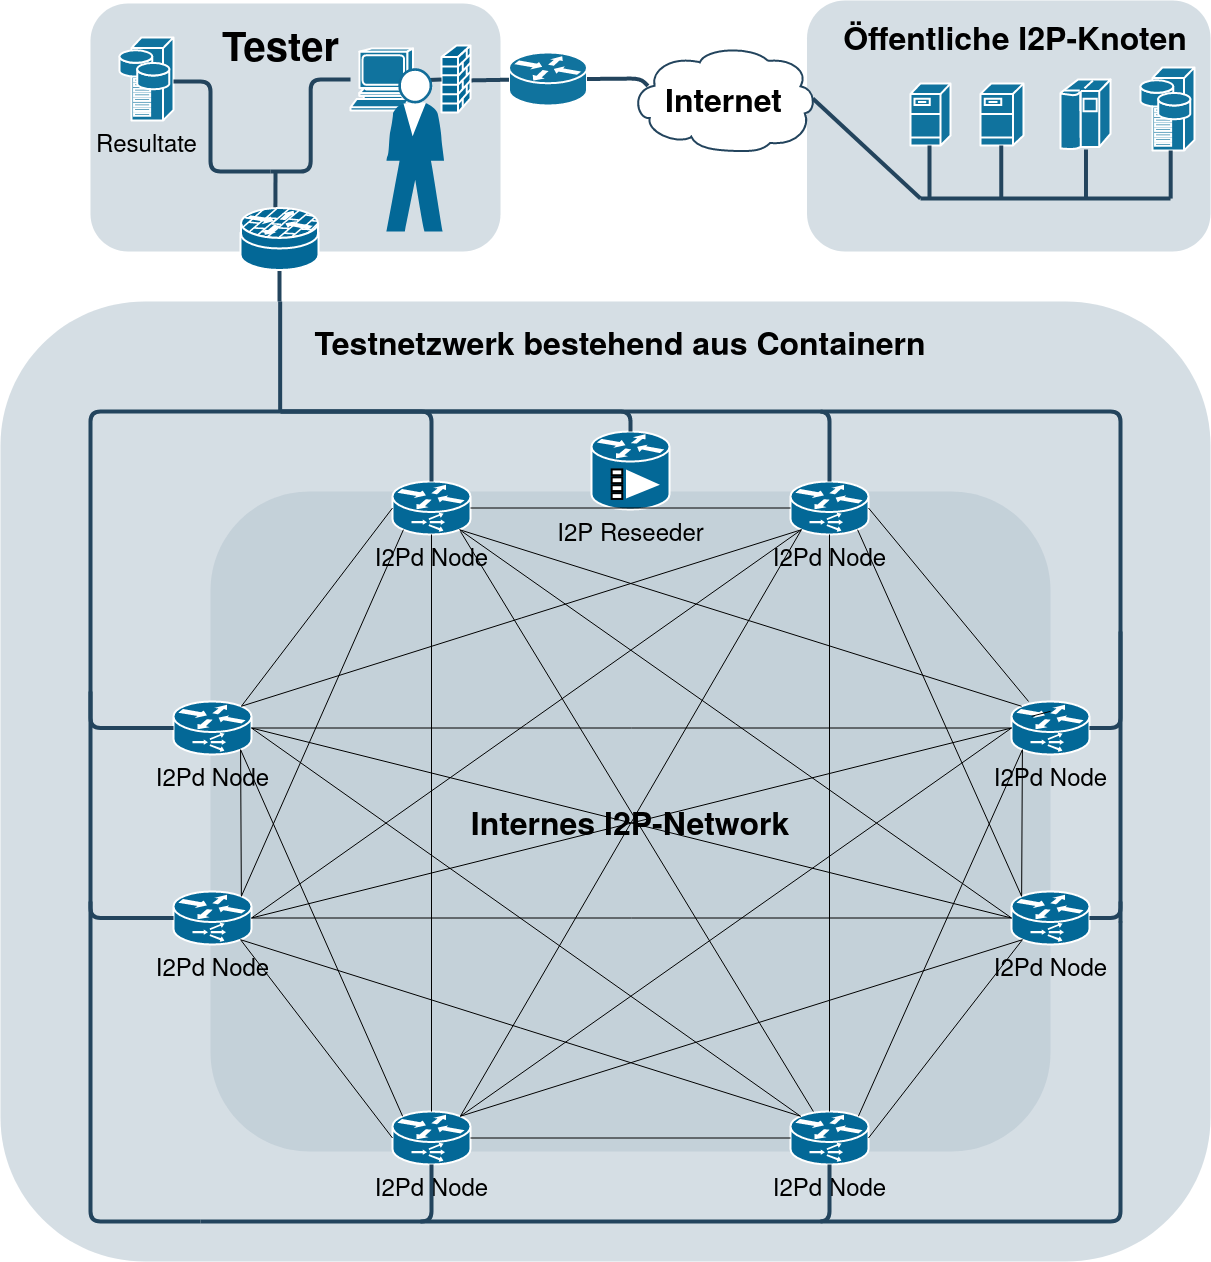
\includegraphics[width=1.0\textwidth]{i2p-testnetwork.png}
\end{figure}


\section{Herausforderungen}

Um ein privates I2P-Testnetzwerk zu erstellen, muss dieses zu Beginn initiiert werden. Dies nennt sich Bootstrap-Vorgang. Dieser Bootstrap-Vorgang erfordert einen eigenen Reseed-Server, welcher die Initialisierungsdaten liefert.
Um die Reproduzierbarkeit von Messungen zu gewährleisten, wurde das Netzwerk automatisiert auf- und abgebaut.
Somit kann dieselbe Messung beliebig oft wiederholt werden.
% Zusätzlich gilt es zu beachten, dass das Testnetzwerk nicht zu viele Ressourcen beansprucht und den Testhost überlastet. Nur so ist es möglich saubere Latenzmessungen zu tätigen die sich wiederholen lassen.

\section{Ergebnisse}

Im Rahmen des Aufbaus der Testumgebung wurden zwei verschiedene Container-Technologien eingesetzt. Zum Einsatz kamen NixOS-Container und Docker-Container.
NixOS-Container beanspruchten zu viele Ressourcen, weswegen schlussendlich Docker-Container eingesetzt wurden .
Damit konnte ein Testnetzwerk bestehend aus bis zu 128 I2P-Knoten erstellt werden.
Somit konnten Latenzmessungen durchgeführt werden,
welche als Grundlage und Referenz für zukünftige Messungen dienen.

\section{Ausblick}

Anhand des entwickelten Teststands können nun weitere Messungen getätigt und miteinander verglichen werden.
Grundsätzlich können so auch verschiedene I2P-Konfigurationen miteinander verglichen werden.
Es sind aber in Zukunft auch Tests mit anderen Protokollen oder Nachrichtentypen möglich.

\end{document}
